%%%%%%%%%%%%%%%%%%%%%%%%%%%%%%%%%%%%%%%%%
% Beamer Presentation
% LaTeX Template
% Version 1.0 (10/11/12)
%
% This template has been downloaded from:
% http://www.LaTeXTemplates.com
%
% License:
% CC BY-NC-SA 3.0 (http://creativecommons.org/licenses/by-nc-sa/3.0/)
%
%%%%%%%%%%%%%%%%%%%%%%%%%%%%%%%%%%%%%%%%%

%----------------------------------------------------------------------------------------
%	PACKAGES AND THEMES
%----------------------------------------------------------------------------------------

\documentclass{beamer}
\usepackage{graphicx}
\usepackage{boxhandler}
\usepackage[utf8]{inputenc}
\usepackage[english]{babel}
\usepackage[Symbol]{upgreek} % recke verze matematickych reckych symbolu
\usepackage{amssymb} % matematické výrazy
\usepackage{amsmath} % matematické výrazy
\usepackage{array}
%\usepackage{textgreek}   % dovolí pužívat up greek pismena
\usepackage{wrapfig}   % text obiha kolem obrazku
\usepackage{caption}   % caption zarovnavani
\usepackage{fancyhdr}  % záhlaví zápatí
\usepackage{gensymb}   % stupne Celsia
\usepackage{subcaption} %for sub figures
\usepackage{mathptmx} %ALICE style J/psi
%\usepackage[style=verbose]{biblatex}
%
%%\bibliographystyle{is-unsrt}


\mode<presentation> {

% The Beamer class comes with a number of default slide themes
% which change the colors and layouts of slides. Below this is a list
% of all the themes, uncomment each in turn to see what they look like.

%\usetheme{default}
%\usetheme{AnnArbor}
%\usetheme{Antibes}
%\usetheme{Bergen}
%\usetheme{Berkeley}
%\usetheme{Berlin}
%\usetheme{Boadilla}
%\usetheme{CambridgeUS}
%\usetheme{Copenhagen}
%\usetheme{Darmstadt}
%\usetheme{Dresden}
%\usetheme{Frankfurt}
%\usetheme{Goettingen}
%\usetheme{Hannover}
%\usetheme{Ilmenau}
%\usetheme{JuanLesPins}
%\usetheme{Luebeck}
\usetheme{Madrid}
%\usetheme{Malmoe}
%\usetheme{Marburg}
%\usetheme{Montpellier}
%\usetheme{PaloAlto}
%\usetheme{Pittsburgh}
%\usetheme{Rochester}
%\usetheme{Singapore}
%\usetheme{Szeged}
%\usetheme{Warsaw}

% As well as themes, the Beamer class has a number of color themes
% for any slide theme. Uncomment each of these in turn to see how it
% changes the colors of your current slide theme.

%\usecolortheme{albatross}
\usecolortheme{beaver}
%\usecolortheme{beetle}
%\usecolortheme{crane}
%\usecolortheme{dolphin}
%\usecolortheme{dove}
%\usecolortheme{fly}
%\usecolortheme{lily}
%\usecolortheme{orchid}
%\usecolortheme{rose}
%\usecolortheme{seagull}
%\usecolortheme{seahorse}
%\usecolortheme{whale}
%\usecolortheme{wolverine}

%\setbeamertemplate{footline} % To remove the footer line in all slides uncomment this line
%\setbeamertemplate{footline}[page number] % To replace the footer line in all slides with a simple slide count uncomment this line

\setbeamertemplate{navigation symbols}{} % To remove the navigation symbols from the bottom of all slides uncomment this line
}

\usepackage{graphicx} % Allows including images
\usepackage{booktabs} % Allows the use of \toprule, \midrule and \bottomrule in tables


%----------------------------------------------------------------------------------------
%	TITLE PAGE
%----------------------------------------------------------------------------------------

\title[]{Parameter error analysis in $\mathrm{J}/\psi$ $\mathrm{p}_\mathrm{\tiny{T}}$ fit} % The short title appears at the bottom of every slide, the full title is only on the title page

\author{Tomáš Herman} % Your name
\institute[FNSPE-CTU] % Your institution as it will appear on the bottom of every slide, may be shorthand to save space
{Faculty of Nuclear Sciences and Physical Engineering \\ Czech Technical University in Prague  }% Your institution for the title page

%\textit{john@smith.com} % Your email address

\date{} 
% Date, can be changed to a custom date, you can set \today


%---------------------------------------------------------------
%####################BEGIN DOCUMENT##########################
%---------------------------------------------------------------
\begin{document}

\begin{frame}
\titlepage % Print the title page as the first slide
\end{frame}

%\begin{frame}
%\frametitle{Outline} % Table of contents slide, comment this block out to remove it
%\tableofcontents % Throughout your presentation, if you choose to use \section{} and \subsection{} commands, these will automatically be printed on this slide as an overview of your presentation
%\end{frame}

%----------------------------------------------------------------------------------------
%	PRESENTATION SLIDES
%----------------------------------------------------------------------------------------


\begin{frame}

\begin{figure}[!ht]
\centering
 {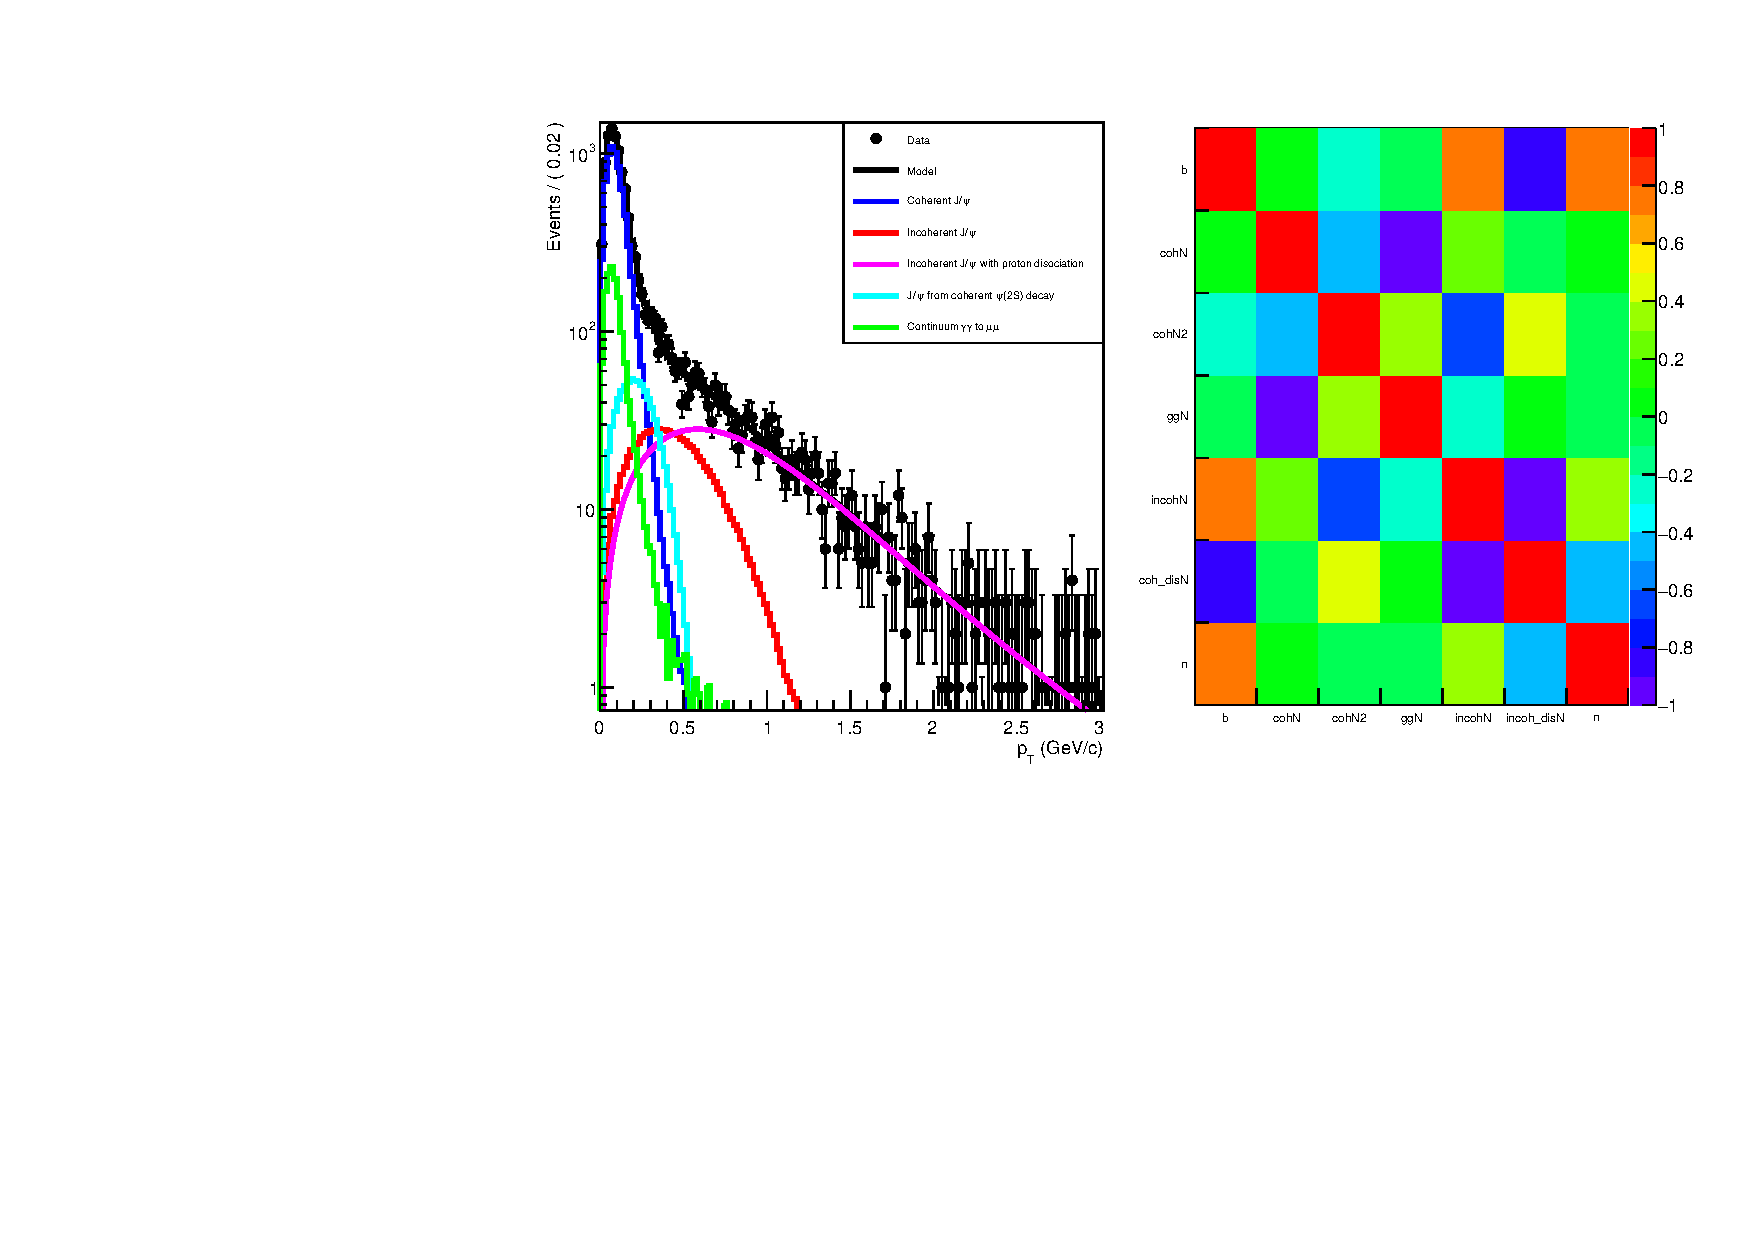
\includegraphics[width=\textwidth]{dataPt_fit.pdf}
\caption{Real data fit, all prameters free.} 
\label{fig:}}
\end{figure}

\end{frame}
\begin{frame}

\begin{table}[!hb]
\begin{center}
\begin{tabular}{|l|r|r|r|}
\hline
\multicolumn{ 2}{|c|}{\textbf{Data}} & \multicolumn{1}{l|}{chi2/ndf:} & 0,835261 \\ \hline
\textbf{Process} & \multicolumn{1}{l|}{\textbf{\#N\_fit}} & \multicolumn{1}{l|}{\textbf{sqrt(\#N\_fit)}} & \multicolumn{1}{l|}{\textbf{\#N\_fit error}} \\ \hline
coh & 6918 & 83 & 645 \\ \hline
incoh & 836 & 29 & 153 \\ \hline
coh2 & 771 & 28 & 106 \\ \hline
gamma & 1352 & 37 & 623 \\ \hline
disoc & 1668 & 41 & 117 \\ \hline
b & 1,6999 & 1,30380 & 1,005736 \\ \hline
n & 3,5661 & 1,88841 & 0,311468 \\ \hline
\end{tabular}
\end{center}
\caption{Real data fit, all prameters free.}
\label{}
\end{table}

\end{frame}
\begin{frame}

\begin{figure}[!ht]
\centering
 {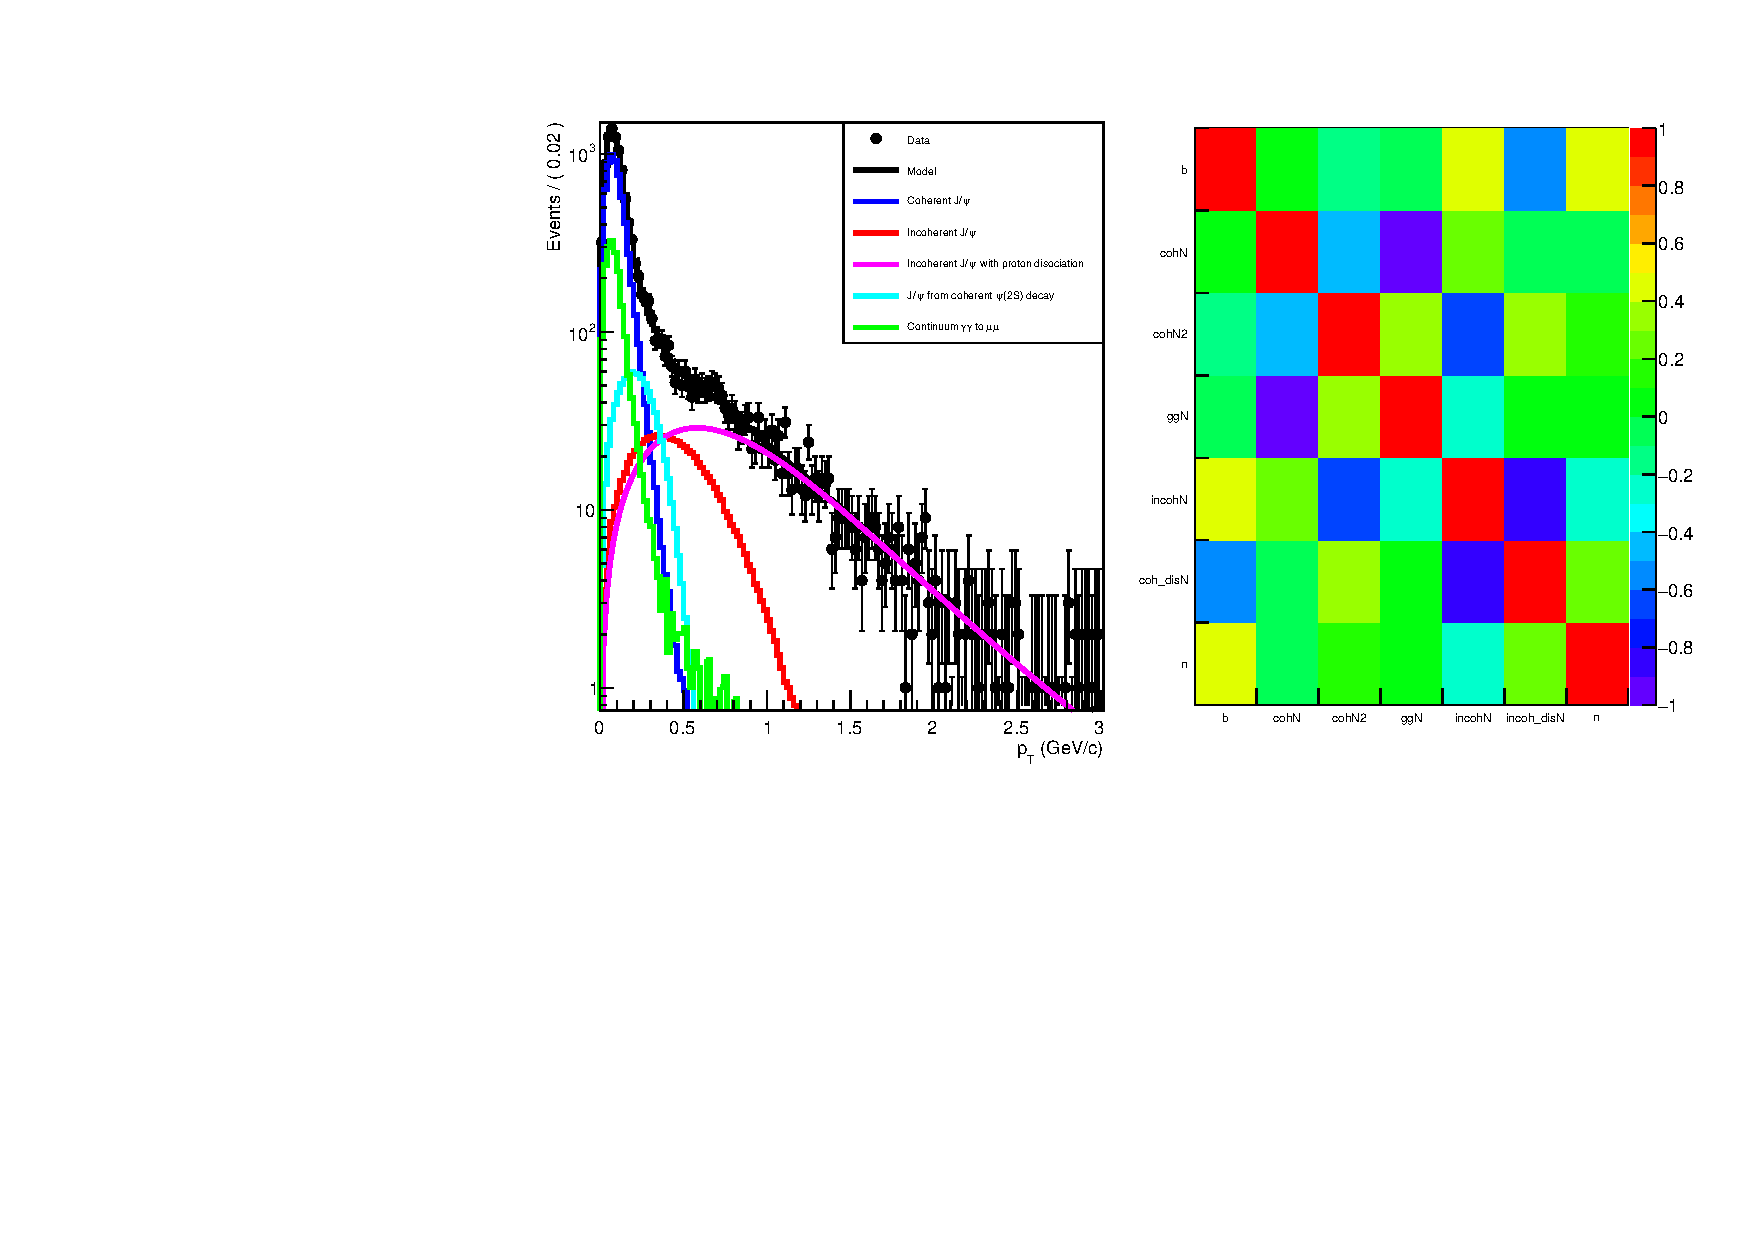
\includegraphics[width=\textwidth]{0Pt_fit.pdf}
\caption{MC data fit, all prameters free.} 
\label{fig:}}
\end{figure}

\end{frame}
\begin{frame}

\begin{table}[!hb]
\begin{center}
\begin{tabular}{|l|r|r|r|r|}
\hline
\multicolumn{3}{|c|}{\textbf{MC data}} & chi2/ndf: & 0,564365 \\ \hline
\textbf{Process} & \multicolumn{1}{l|}{\textbf{\#entries}} & \multicolumn{1}{l|}{\textbf{\#N\_fit}} & \multicolumn{1}{l|}{\textbf{sqrt(\#N\_fit)}} & \multicolumn{1}{l|}{\textbf{\#N\_fit error}} \\ \hline
coh & 6882 & 6245 & 79 & 643 \\ \hline
incoh & 852 & 775 & 28 & 133 \\ \hline
coh2 & 721 & 847 & 29 & 104 \\ \hline
gamma & 1350 & 1927 & 44 & 622 \\ \hline
disoc & 1668 & 1677 & 41 & 98 \\ \hline
b & 1,7 & 1,7 & 1,30384 & 0,0957796 \\ \hline
n & 3,56 & 3,766 & 1,94062 & 0,283356 \\ \hline
\end{tabular}
\end{center}
\caption{MC data fit, all prameters free.}
\label{}
\end{table}



\end{frame}
\begin{frame}

\begin{figure}[!ht]
\centering
 {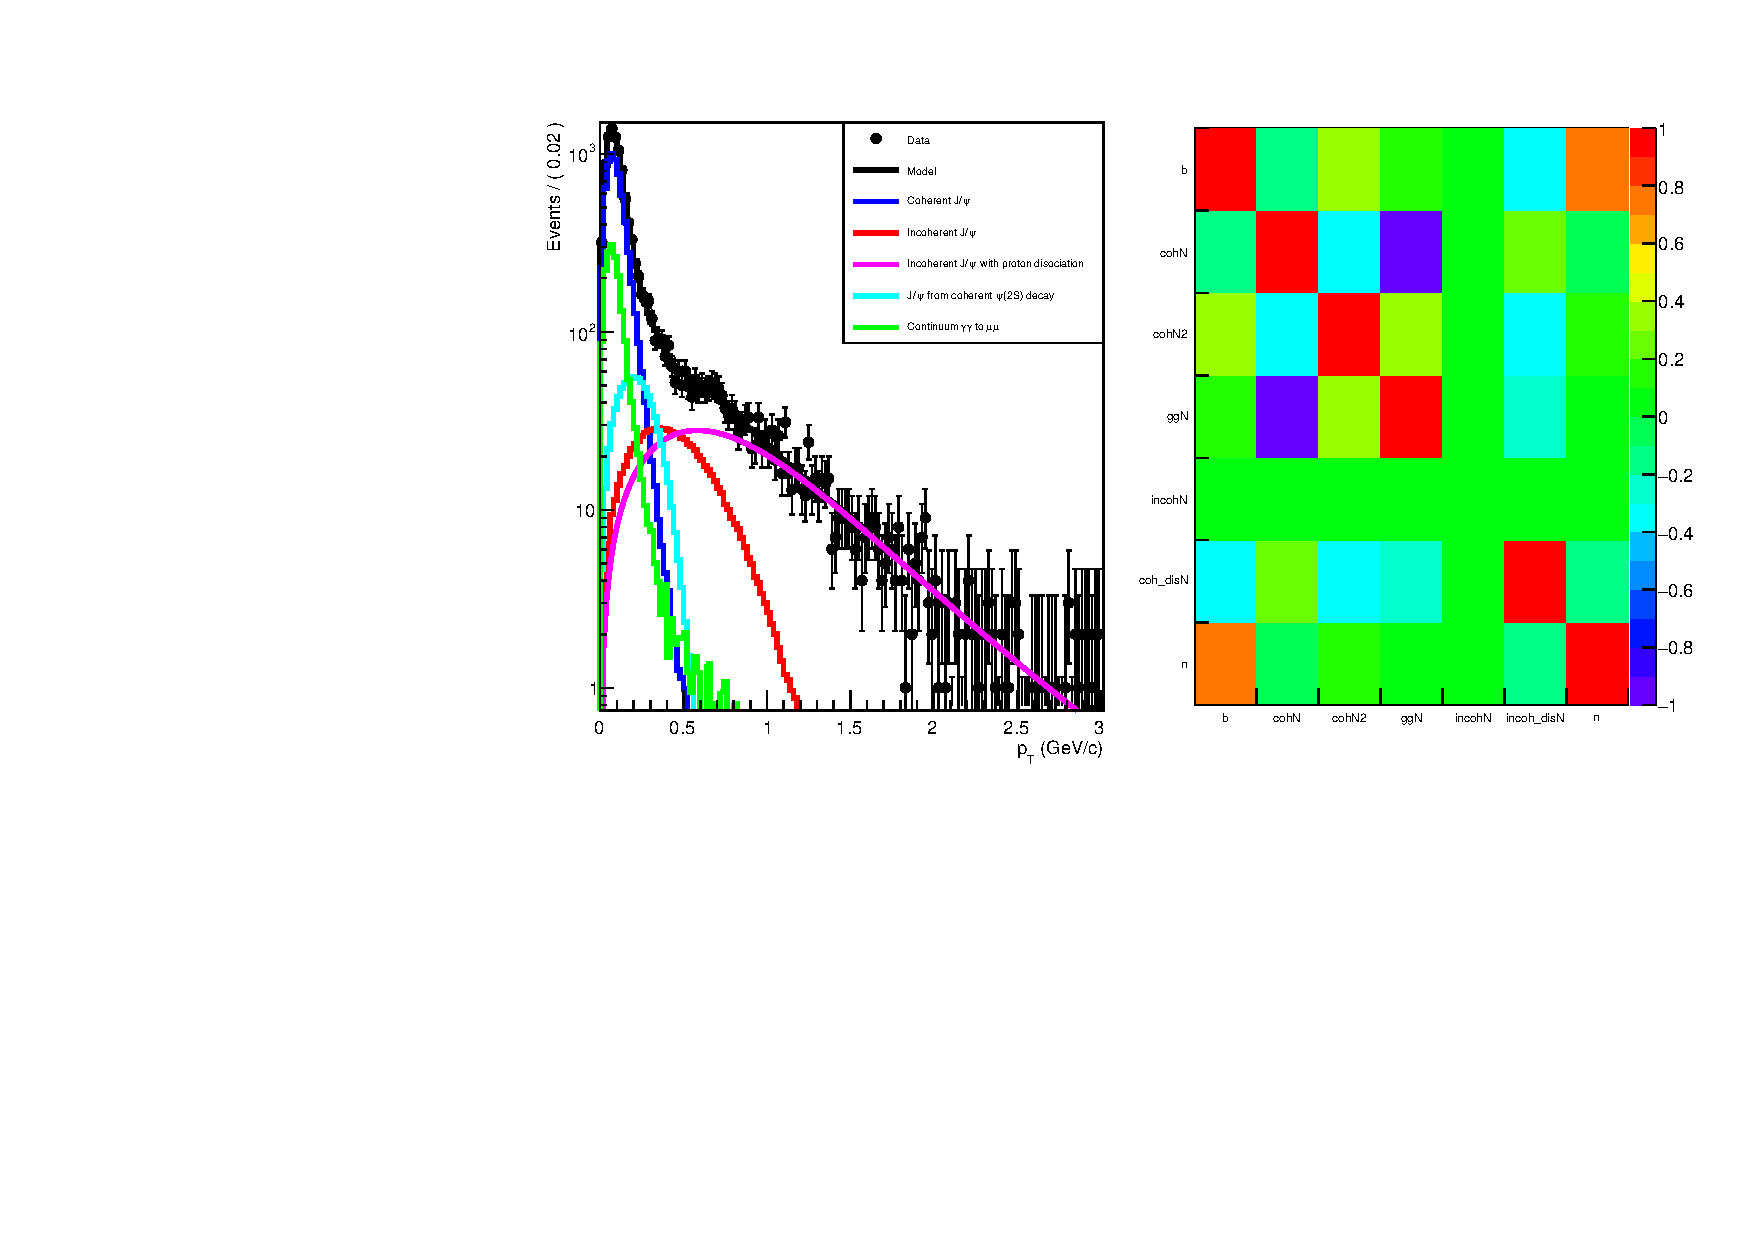
\includegraphics[width=\textwidth]{1Pt_fit.pdf}
\caption{MC data fit, incoh fixed.} 
\label{fig:}}
\end{figure}

\end{frame}
\begin{frame}

\begin{table}[!hb]
\begin{center}
\begin{tabular}{|l|r|r|r|r|}
\hline
\multicolumn{3}{|c|}{\textbf{MC data}} & chi2/ndf: & 0,56137 \\ \hline
\textbf{Process} & \multicolumn{1}{l|}{\textbf{\#entries}} & \multicolumn{1}{l|}{\textbf{\#N\_fit}} & \multicolumn{1}{l|}{\textbf{sqrt(\#N\_fit)}} & \multicolumn{1}{l|}{\textbf{\#N\_fit error}} \\ \hline
coh & 6882 & 6367 & 80 & 624 \\ \hline
incoh & 852 & \multicolumn{1}{l|}{fixed} & \#VALUE! & \multicolumn{1}{l|}{} \\ \hline
coh2 & 721 & 803 & 28 & 83 \\ \hline
gamma & 1350 & 1817 & 43 & 607 \\ \hline
disoc & 1668 & 1636 & 40 & 59 \\ \hline
b & 1,7 & 1,7 & 1,30384 & 0,131825 \\ \hline
n & 3,56 & 3,67379 & 1,91671 & 0,319593 \\ \hline
\end{tabular}
\end{center}
\caption{MC data fit, incoh fixed.}
\label{}
\end{table}

\end{frame}
\begin{frame}

\begin{figure}[!ht]
\centering
 {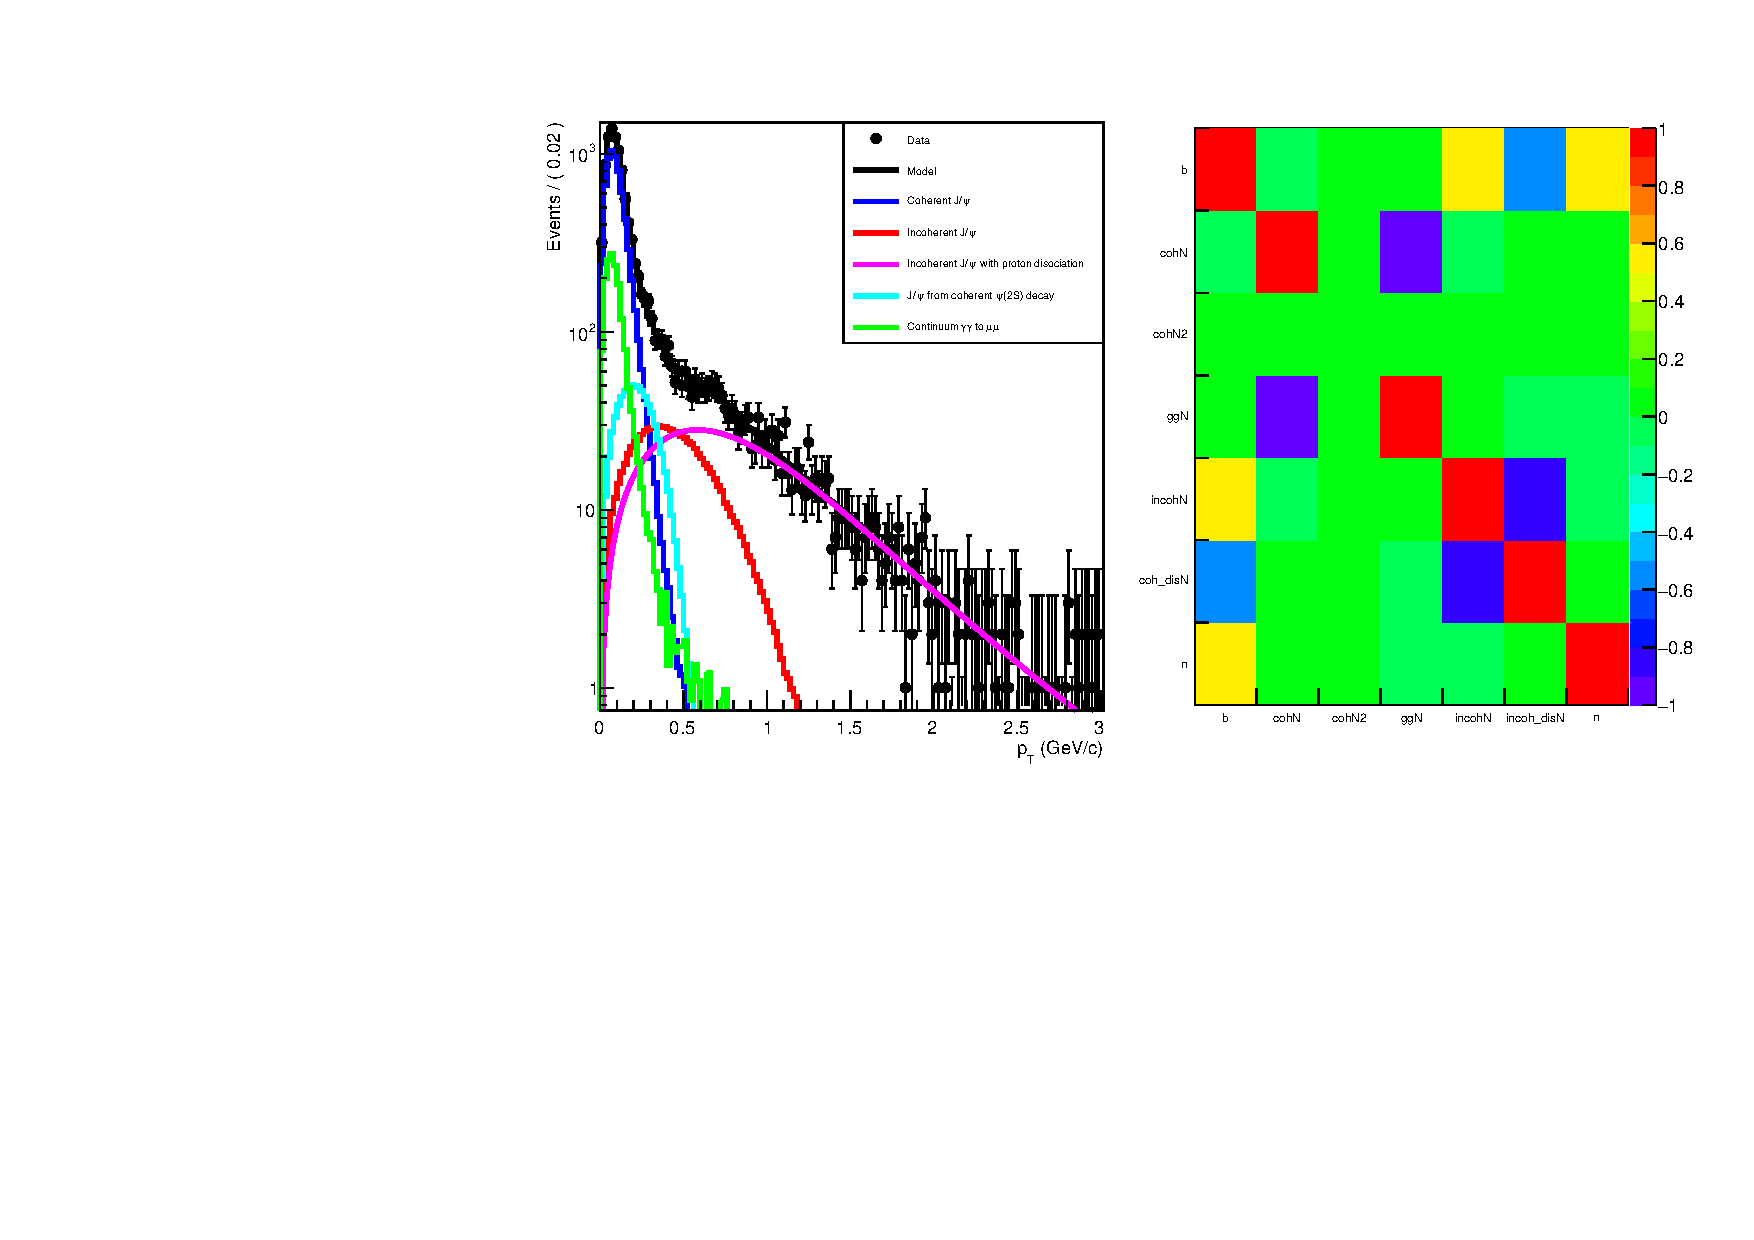
\includegraphics[width=\textwidth]{2Pt_fit.pdf}
\caption{MC data fit, coh2 fixed.} 
\label{fig:}}
\end{figure}

\end{frame}
\begin{frame}

\begin{table}[bp]
\begin{center}
\begin{tabular}{|l|r|r|r|r|}
\hline
\multicolumn{3}{|c|}{\textbf{MC data}} & chi2/ndf: & 0,569302 \\ \hline
\textbf{Process} & \multicolumn{1}{l|}{\textbf{\#entries}} & \multicolumn{1}{l|}{\textbf{\#N\_fit}} & \multicolumn{1}{l|}{\textbf{sqrt(\#N\_fit)}} & \multicolumn{1}{l|}{\textbf{\#N\_fit error}} \\ \hline
coh & 6882 & 6601 & 81 & 575 \\ \hline
incoh & 852 & 870 & 29 & 107 \\ \hline
coh2 & 721 & \multicolumn{1}{l|}{fixed} & \#VALUE! & \multicolumn{1}{l|}{} \\ \hline
gamma & 1350 & 1629 & 40 & 574 \\ \hline
disoc & 1668 & 1642 & 41 & 95 \\ \hline
b & 1,7 & 1,7 & 1,30384 & 0,124875 \\ \hline
n & 3,56 & 3,69064 & 1,92110 & 0,28677 \\ \hline
\end{tabular}
\end{center}
\caption{MC data fit, coh2 fixed.}
\label{}
\end{table}
\end{frame}
\begin{frame}

\begin{figure}[!ht]
\centering
 {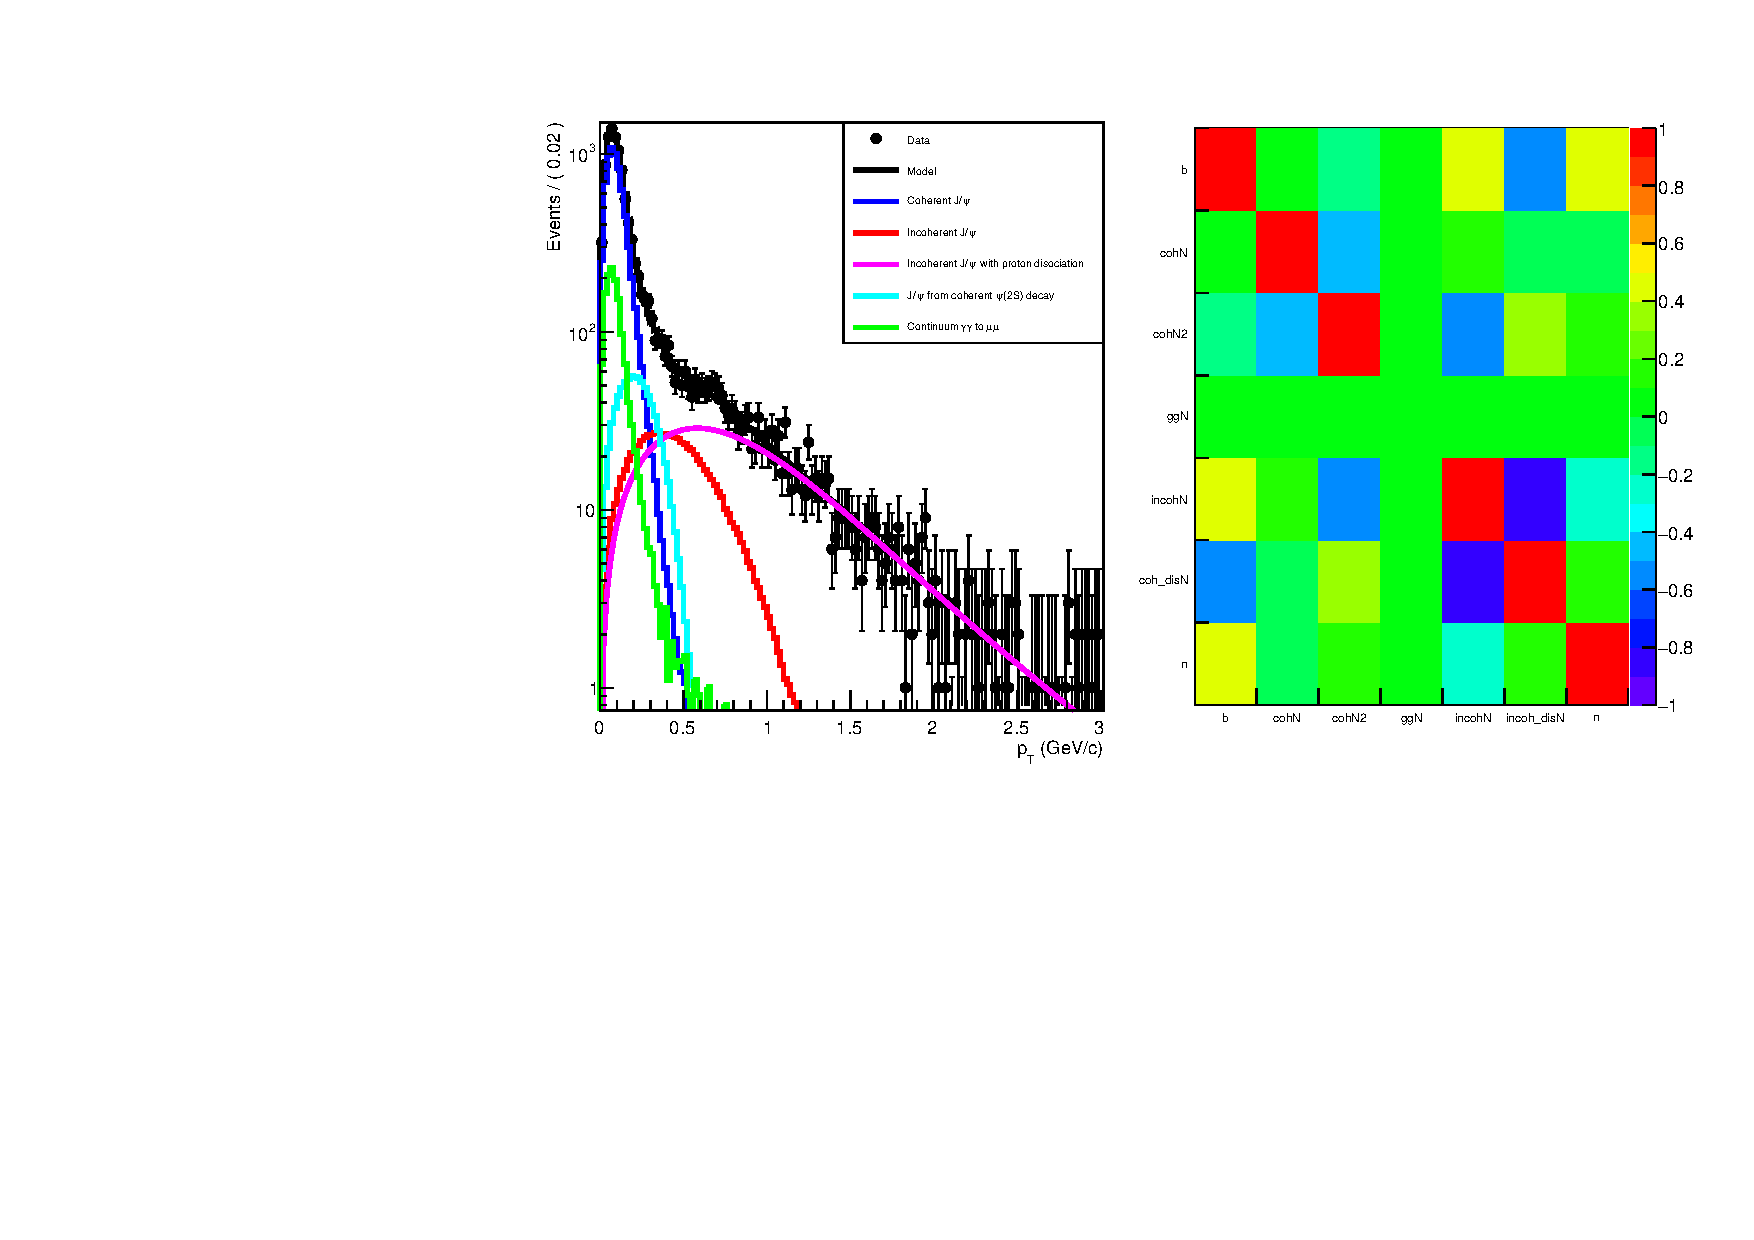
\includegraphics[width=\textwidth]{3Pt_fit.pdf}
\caption{MC data fit, gamma fixed.} 
\label{fig:}}
\end{figure}

\end{frame}
\begin{frame}

\begin{table}[bp]
\begin{center}
\begin{tabular}{|l|r|r|r|r|}
\hline
\multicolumn{3}{|c|}{\textbf{MC data}} & chi2/ndf: & 0,5631 \\ \hline
\textbf{Process} & \multicolumn{1}{l|}{\textbf{\#entries}} & \multicolumn{1}{l|}{\textbf{\#N\_fit}} & \multicolumn{1}{l|}{\textbf{sqrt(\#N\_fit)}} & \multicolumn{1}{l|}{\textbf{\#N\_fit error}} \\ \hline
coh & 6882 & 6833 & 83 & 107 \\ \hline
incoh & 852 & 804 & 28 & 129 \\ \hline
coh2 & 721 & 810 & 28 & 96 \\ \hline
gamma & 1350 & \multicolumn{1}{l|}{fixed} & \#VALUE! & \multicolumn{1}{l|}{} \\ \hline
disoc & 1668 & 1672 & 41 & 98 \\ \hline
b & 1,7 & 1,7 & 1,30384 & 0,10194 \\ \hline
n & 3,56 & 3,7533 & 1,93734 & 0,283619 \\ \hline
\end{tabular}
\end{center}
\caption{MC data fit, gamma fixed.}
\label{}
\end{table}

\end{frame}
\begin{frame}


\begin{figure}[!ht]
\centering
 {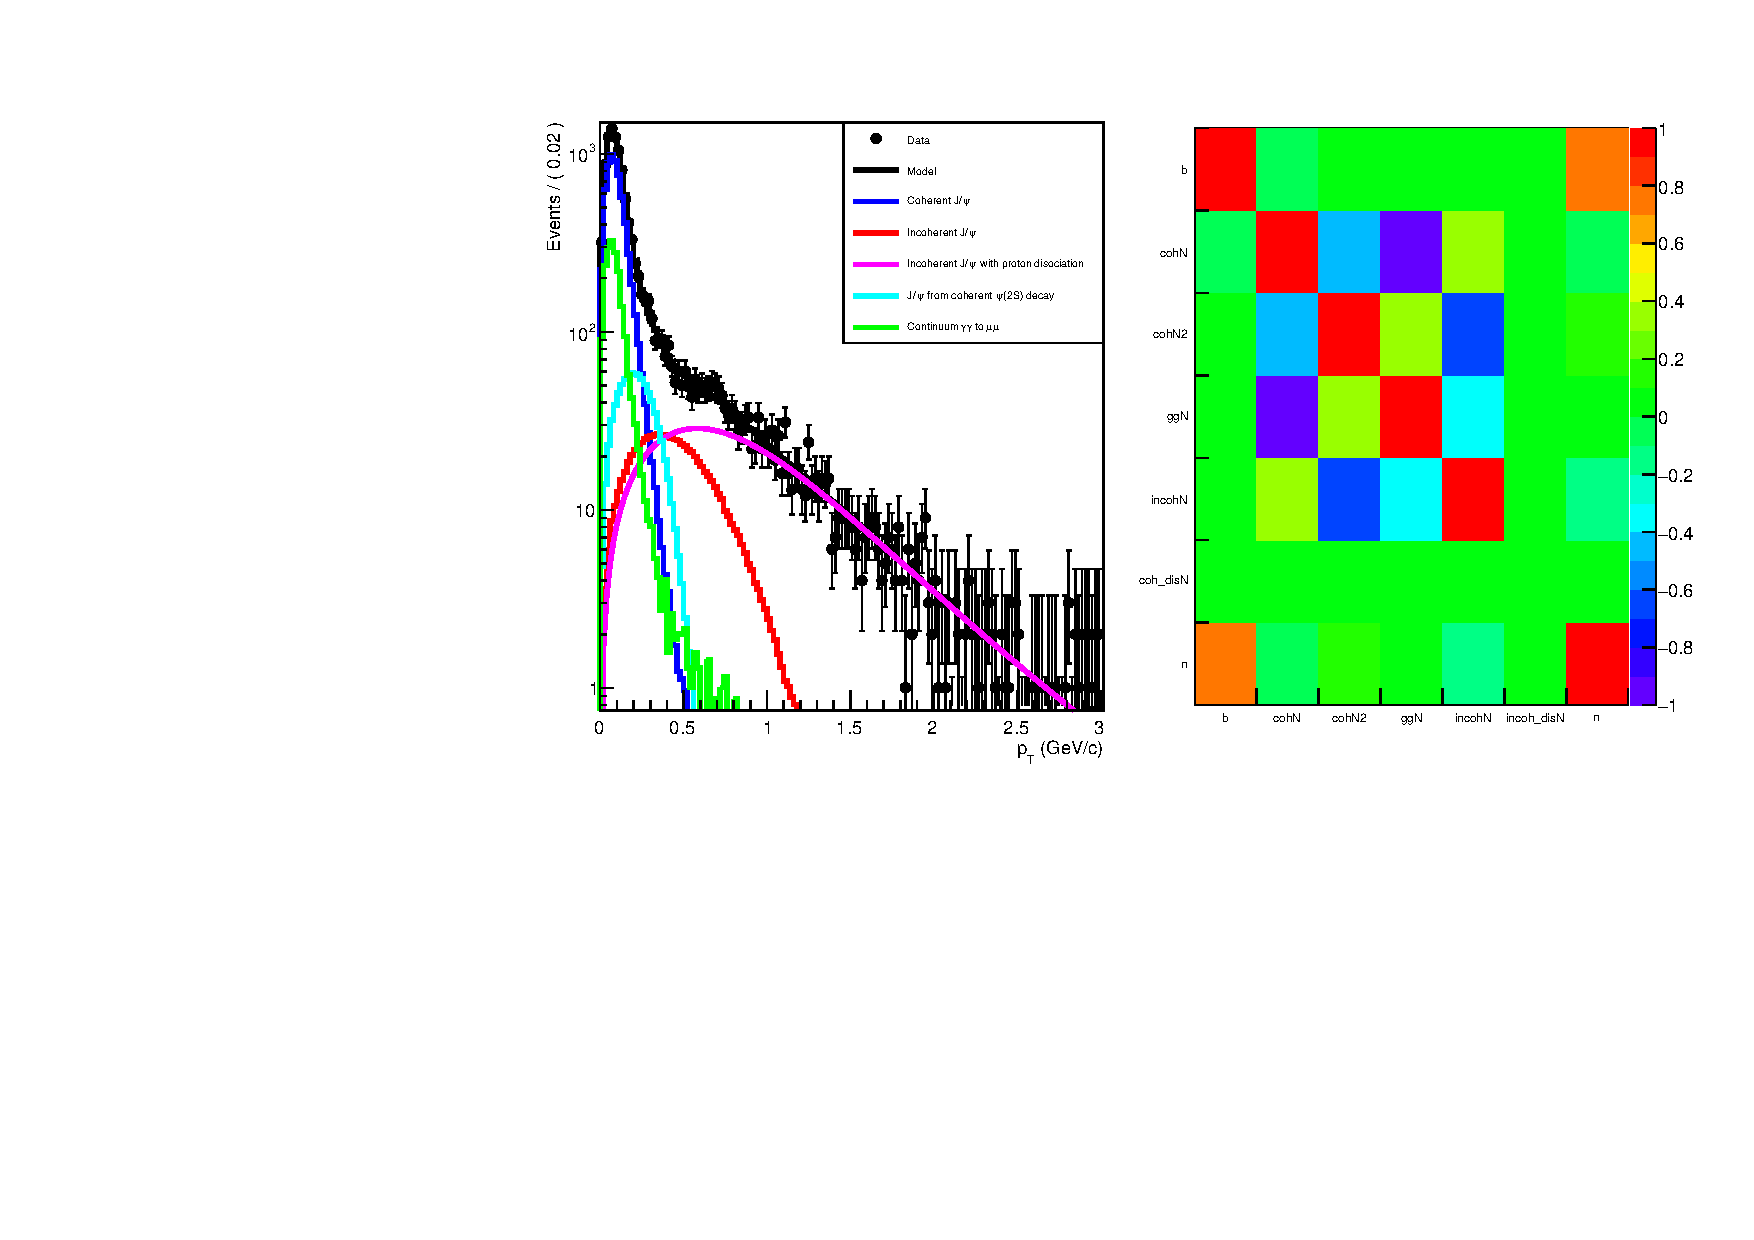
\includegraphics[width=\textwidth]{4Pt_fit.pdf}
\caption{MC data fit, disoc fixed.} 
\label{fig:}}
\end{figure}

\end{frame}
\begin{frame}

\begin{table}[bp]
\begin{center}
\begin{tabular}{|l|r|r|r|r|}
\hline
\multicolumn{3}{|c|}{\textbf{MC data}} & chi2/ndf: & 0,5631 \\ \hline
\textbf{Process} & \multicolumn{1}{l|}{\textbf{\#entries}} & \multicolumn{1}{l|}{\textbf{\#N\_fit}} & \multicolumn{1}{l|}{\textbf{sqrt(\#N\_fit)}} & \multicolumn{1}{l|}{\textbf{\#N\_fit error}} \\ \hline
coh & 6882 & 6250 & 79 & 641 \\ \hline
incoh & 852 & 785 & 28 & 77 \\ \hline
coh2 & 721 & 843 & 29 & 98 \\ \hline
gamma & 1350 & 1923 & 44 & 621 \\ \hline
disoc & 1668 & \multicolumn{1}{l|}{fixed} & \#VALUE! & \multicolumn{1}{l|}{} \\ \hline
b & 1,7 & 1,7 & 1,30384 & 0,0795964 \\ \hline
n & 3,56 & 3,75047 & 1,93661 & 0,285092 \\ \hline
\end{tabular}
\end{center}
\caption{MC data fit, disoc fixed.}
\label{}
\end{table}

\end{frame}

\end{document}





 
 








